% Uncomment this line for on-screen presentation
\documentclass[xcolor={dvipsnames}]{beamer}\usepackage{etoolbox}\newtoggle{printable}\togglefalse{printable}

% Uncomment this line for printable slides (disable animations and don't waste ink)
%\documentclass[handout, xcolor={dvipsnames}]{beamer}\usepackage{etoolbox}\newtoggle{printable}\toggletrue{printable}

% Adjust these for the path of the theme and its graphics, relative to this file
%\usepackage{beamerthemeFalmouthGamesAcademy}
\usepackage{../../beamerthemeFalmouthGamesAcademy}
\graphicspath{ {../../} }

% Default language for code listings
\lstset{language=C++,
		morekeywords={each,in}
}

\begin{document}
\title{Programming Practice III}   
\subtitle{BSc Computing for Games}

\frame{\titlepage} 

\part{Morning}
\frame{\partpage}

\begin{frame}{Hardware Hacking}
	In this morning's session you will:
	
	\begin{itemize}
		\item Self-organise into \textbf{TWO} groups
		\item As a group, \textbf{complete} the online MakeyMakey tutorials
		\item As a group, \textbf{complete} the tutorials in Sunfounder Arduino Kit tutorials
		\item After completing the tutorials, as individuals, continue \textbf{developing} your game controller prototypes
	\end{itemize}
\end{frame}

\part{Afternoon}
\frame{\partpage}

\begin{frame}{Sprint Reviews and Team Meetings}
	In the afternoon session you will:
	
	\begin{itemize}
		\item \textbf{Prepare} for your sprint review by \textbf{assembling} the prototype and \textbf{updating} the Trello board.
		\item Sprint reviews will commence at 3pm
		\item \textbf{Conduct} a meeting with your COMP150 group. In this meeting, you should focus on the:
		\begin{itemize}
			\item Group name
			\item Commercial goals
			\item Design goals
			\item Management issues
		\end{itemize}
	\end{itemize}
\end{frame}

% -------------------------------------------------------

%\part{The compiler}
%\frame{\partpage}
%
%\begin{frame}
%	\frametitle{The build process}
%	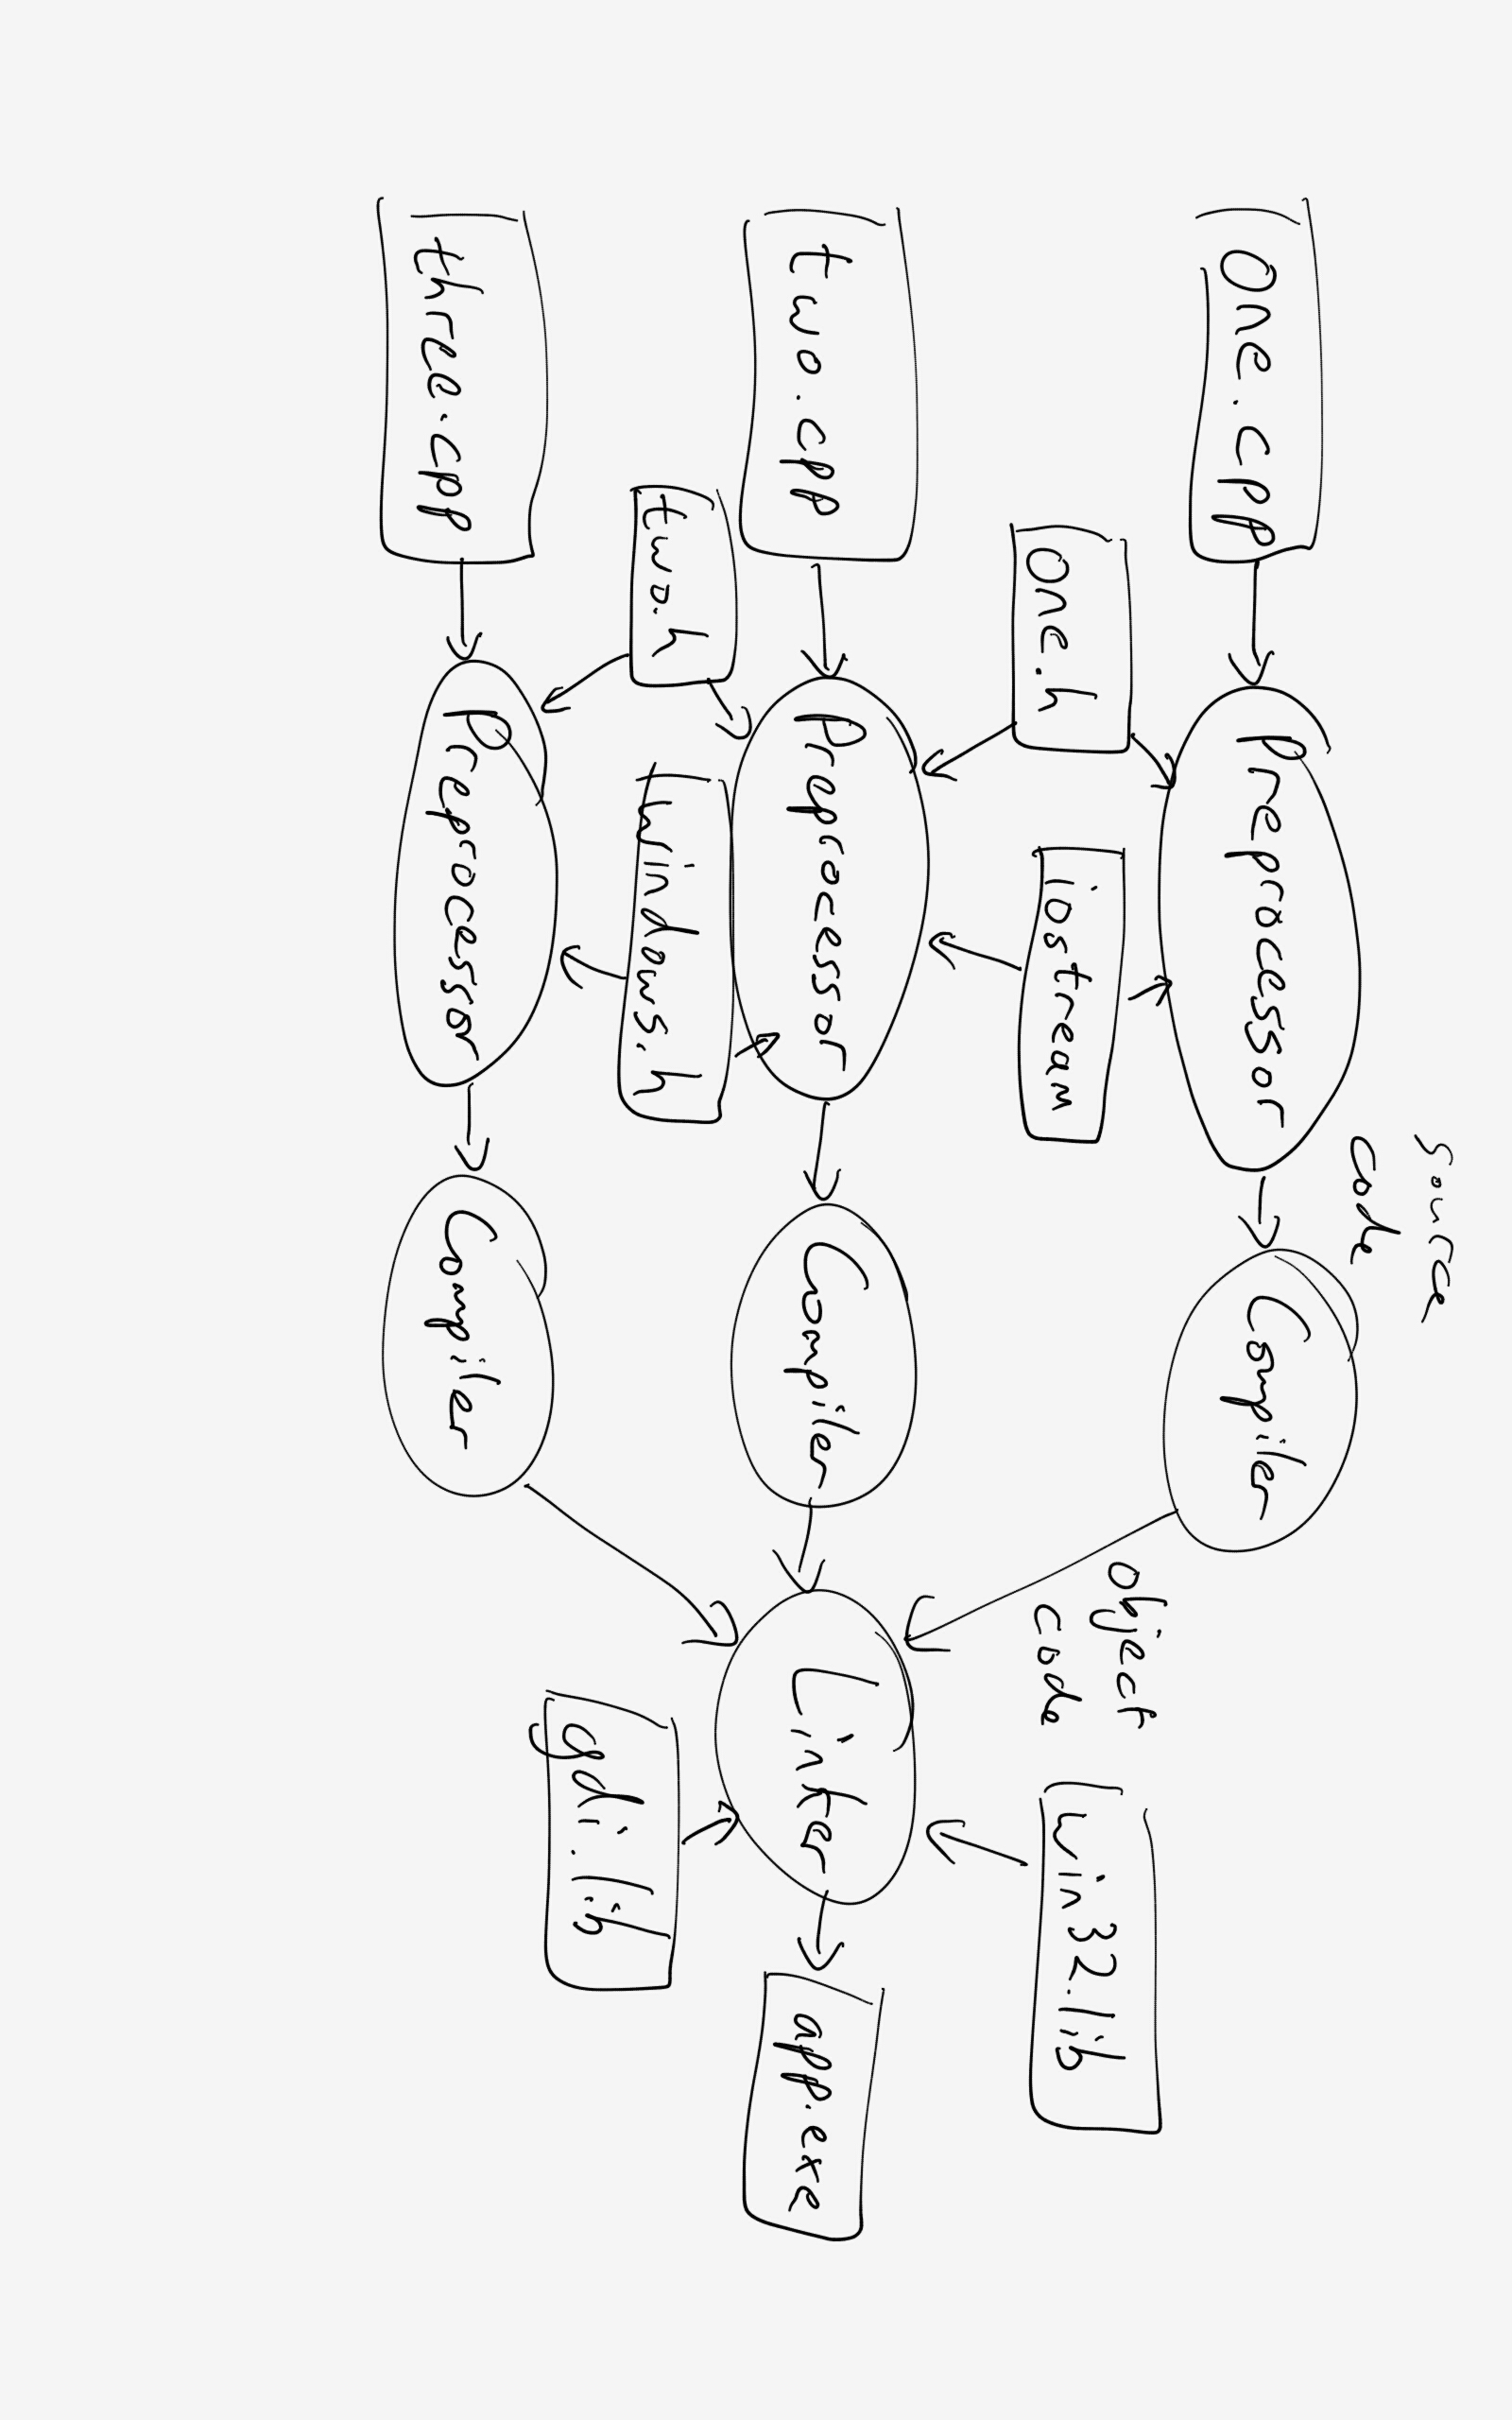
\includegraphics[height=\textwidth,angle=90]{compiler_sketch}
%\end{frame}

\end{document}
